\chapter{Contexto Histórico}
\section{Época de los Tres Reinos de la península coreana}

La \textbf{época de los Tres Reinos} en Corea es un período histórico crucial que se extendió desde aproximadamente el siglo I hasta el siglo VII d.C. Durante este tiempo, la península coreana estaba dividida en tres reinos principales, cada uno con sus propias características y contribuciones a la historia y cultura de Corea.

\begin{figure}[h]
	\centering
	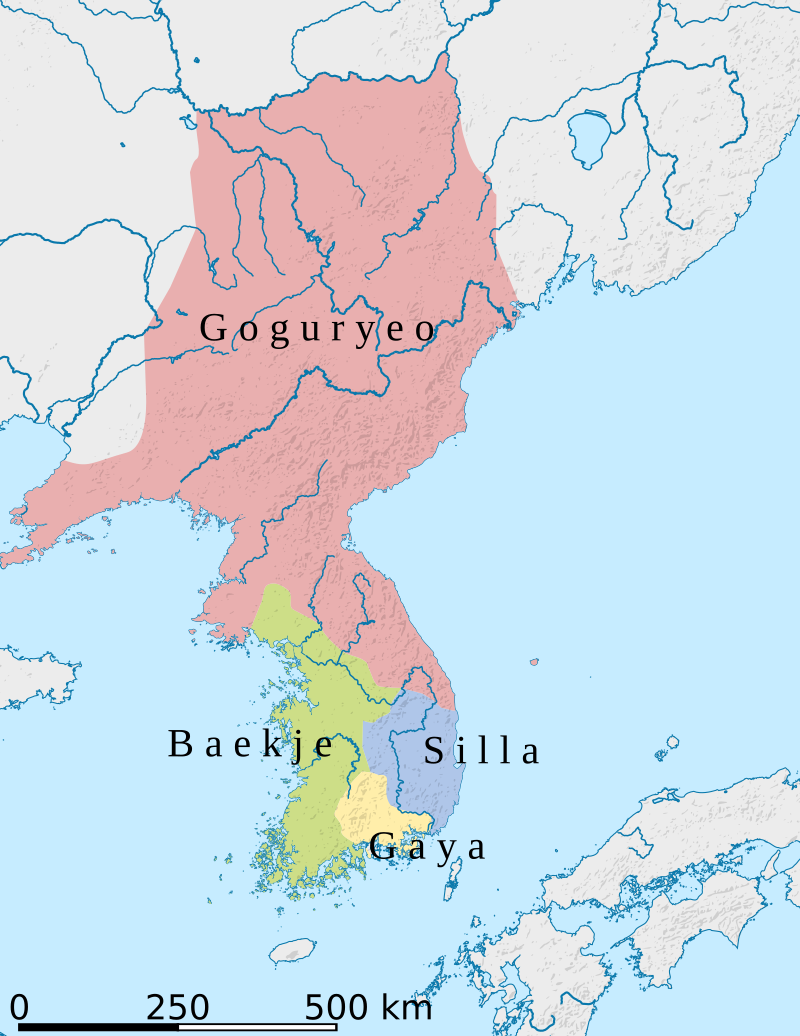
\includegraphics[width=0.3\textwidth]{images/Historia/mapa_tres_reinos.png} % Reemplaza 'mapa_corea' con el nombre de tu archivo de imagen
	\caption{Mapa de Corea con los Tres Reinos}
\end{figure}

\subsection{Goguryeo}

Goguryeo fue el reino más septentrional y poderoso de los Tres Reinos. Su capital estaba ubicada en la actual región norcoreana. Goguryeo mantuvo una fuerte influencia militar y política en la península, y se caracterizó por su habilidad para resistir las invasiones chinas de la dinastía Han y luego de la dinastía Tang. Este reino desarrolló una cultura propia y estableció una gran parte de lo que hoy es Corea del Norte.

\subsection{Baekje}

Baekje ocupó la región suroeste de la península coreana, con su capital en lo que hoy es la ciudad de Seúl. Este reino tenía estrechos vínculos culturales y comerciales con China y Japón, lo que le permitió adoptar y difundir la influencia budista en la península. Baekje fue conocido por su avanzada cultura y arte, y contribuyó significativamente al desarrollo de la cultura coreana.

\subsection{Silla}

Silla, ubicado en la región sureste de Corea con su capital en Gyeongju, fue el último de los Tres Reinos en unificarse bajo un gobierno centralizado. Silla es famoso por su sistema de gobierno estable y su énfasis en la educación y la cultura. Durante esta época, se estableció el sistema de exámenes gubernamentales basado en el conocimiento confuciano, que influyó en gran medida en la administración pública de Corea durante siglos.

A medida que avanzaba la época de los Tres Reinos, se produjo una serie de conflictos y alianzas cambiantes entre los reinos, con episodios de unificación temporal y fragmentación. Finalmente, en el siglo VII, Silla logró unificar la península coreana bajo su dominio y estableció el período conocido como el ''Silla Unificado``. Este período dio paso a una mayor estabilidad y desarrollo cultural en Corea antes de la llegada de la dinastía Goryeo. La época de los Tres Reinos dejó un profundo legado en la historia y la cultura de Corea, con influencias que perduran hasta el día de hoy.

\section{Hwarang}

Los \textbf{Hwarang}, también conocidos como ''Hwa Rang`` o ''Hwarangdo\textregistered``, fueron un grupo de jóvenes guerreros aristocráticos en la antigua Corea. Su existencia se sitúa en los períodos de los Tres Reinos y la posterior dinastía Silla, que abarcan los siglos VI al X d.C. Estos guerreros eran conocidos no sólo por su habilidad en el combate, sino también por su énfasis en la educación, la moral, la cultura y las artes.

\begin{figure}[h]
	\centering
	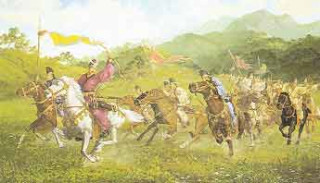
\includegraphics[width=0.3\textwidth]{images/Historia/pintura_hrd.jpg} % Reemplaza 'mapa_corea' con el nombre de tu archivo de imagen
	\caption{Grupo élite de Corea}
\end{figure}


\subsubsection{Origen y Significado}

La palabra ''Hwarang`` se traduce aproximadamente como ``caballeros de la flor'' o ``juventud floreciente''. Eran un grupo selecto de jóvenes nobles que se sometían a un entrenamiento riguroso tanto en artes marciales como en aspectos culturales y éticos.

\subsubsection{Educación Integral}

Los Hwarang no solo se entrenaban en técnicas de combate, sino que también recibían una educación completa que incluía poesía, música, filosofía y moral. Este enfoque en la educación y la cultura los diferenciaba de otros guerreros de la época.

\subsubsection{Código de Ética}

\begin{table}[t]
	\caption{Código Hwarang}
	\begin{center}
		\begin{tabular}{ | m{2cm} | m{5cm} | m{5cm} | }
			\hline Número & Hangul & Traducción \\ \hline
			Il & 사군이충: Sa Gun I Chung & Lealtad a nuestra Patria \\
			I & 사친이효: Sa Chin I Hyo & Lealtad a nuestros padres y maestros \\
			Sam & 교우이신: Gyo U I Sin & Confianza y hermandad entre amigos\\
			Sa & 임전무퇴: Im Jeon Mu Toe & Coraje para no retroceder frente al enemigo\\
			O & 살생유택: Sal Saeng Yu Taek & Justicia para no tomar una vida sin causa\\ \hline
		\end{tabular}
	\end{center}
\end{table}


Los Hwarang seguían un estricto código de ética conocido como ''Hwarangdo\textregistered``, que promovía valores como la lealtad, la rectitud, la valentía y la integridad. Este código tenía como objetivo formar no solo guerreros hábiles, sino también líderes virtuosos.

El fervor de los Hwarang ayudó a que Silla se convirtiera en la primera ''Tierra de Buda`` del mundo y condujo a la unificación de los tres reinos de Corea. Los principios budistas estaban tan arraigados en el código de los Hwarang que un gran número de monjes participaba en el Hwarang-Do, y durante tiempos de guerra, se despojaban de sus hábitos y tomaban las armas para morir por Silla.

El código Hwarang fue establecido en el trigésimo año del reinado del Rey Chin-Hung. Dos destacados guerreros Hwarang, Kwi-San y Ch'u-Hang, buscaron al famoso guerrero y monje budista Wong-Gwang Popsa en el Templo Kusil en la Montaña Unmun y le pidieron que les diera mandamientos que los hombres pudieran seguir y que no abrazaran la vida recluida de un monje budista.

\begin{figure}[h]
	\centering
	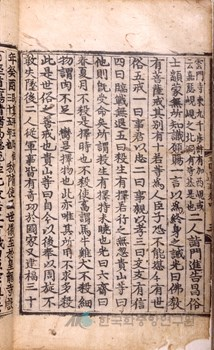
\includegraphics[width=0.4\textwidth]{images/Historia/codigo_hwarang.jpg} % Reemplaza 'mapa_corea' con el nombre de tu archivo de imagen
	\caption{Las Cinco Reglas Seculares de la Escuela de Wongwang en la época de los 3 reinos}
\end{figure}

Los mandamientos, basados en principios confucianos y budistas, se dividieron en el Código de las cinco reglas Hwarang y las nueve virtudes. Estos principios no eran tomados a la ligera por los Hwarang.


\begin{table}[t]
	\caption{Nueve Virtudes}
	\begin{center}
		\begin{tabular}{ | m{2cm} | m{5cm} | }
			\hline Hangul & Traducción \\ \hline
			인: In & Humanidad \\
			의: Ui & Justicia \\
			예: Ye & Cortesía \\
			지: Ji & Sabiduría \\
			신: Sin & Confianza \\
			선: Seon & Bondad \\
			덕: Deok & Virtud \\
			충: Chung & Lealtad \\
			용: Yong & Coraje \\

			\hline
		\end{tabular}
	\end{center}
\end{table}


El fervor de los Hwarang ayudó a que Silla se convirtiera en la primera "Tierra de Buda" del mundo y condujo a la unificación de los tres reinos de Corea. Los principios budistas estaban tan arraigados en el código de los Hwarang que un gran número de monjes participaban en el Hwarang-Do, y durante tiempos de guerra, se despojarían de sus hábitos y tomarían las armas para morir por Silla.

\subsubsection{Artes Marciales}

Aunque se destacaban en la educación y la cultura, los Hwarang también eran conocidos por su habilidad en el combate. Dominaban varias formas de artes marciales y estaban preparados para defender su reino en caso de guerra.

\subsubsection{Contribución a la Unificación de Silla}

Durante el período de los Tres Reinos en Corea, Silla se convirtió en uno de los reinos más poderosos. Se dice que los Hwarang desempeñaron un papel crucial en la unificación de Silla y en la posterior estabilidad del reino.

\subsubsection{Legado Cultural}

La influencia de los Hwarang perduró en la cultura coreana a lo largo de la historia. Su énfasis en la educación, la ética y la excelencia en las artes marciales influyó en la formación de la cultura y la identidad coreanas.

Los Hwarang son un ejemplo único en la historia de las sociedades guerreras, ya que combinaron la destreza en el combate con un profundo compromiso con la educación y los valores morales. Su legado sigue siendo un símbolo importante de la historia y la cultura coreanas.


%\begin{figure}[h]
%	\centering
%
%	\subfloat[Imagen 1]{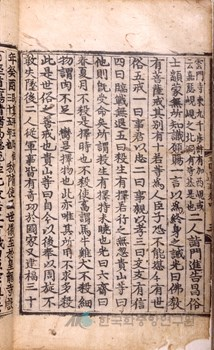
\includegraphics[width=0.2\textwidth]{images/Historia/codigo_hwarang.jpg}}\hspace{1cm}
%	\subfloat[Imagen 2]{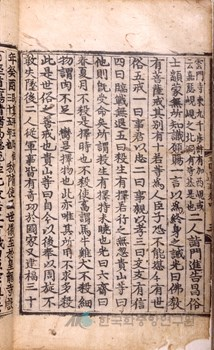
\includegraphics[width=0.2\textwidth]{images/Historia/codigo_hwarang.jpg}}\hspace{1cm}
%	\subfloat[Imagen 3]{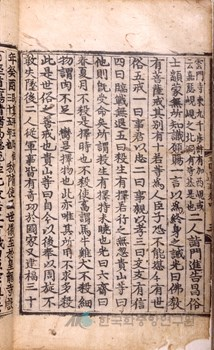
\includegraphics[width=0.2\textwidth]{images/Historia/codigo_hwarang.jpg}}\hspace{1cm}
%	\subfloat[Imagen 4]{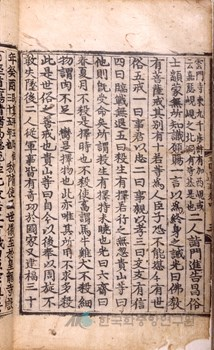
\includegraphics[width=0.2\textwidth]{images/Historia/codigo_hwarang.jpg}}\hspace{1cm}
%	\subfloat[Imagen 5]{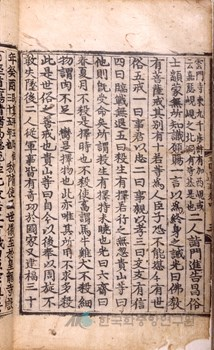
\includegraphics[width=0.2\textwidth]{images/Historia/codigo_hwarang.jpg}}
%
%	\caption{Secuencia Patada Frontal}
%
%\end{figure}
